\documentclass[1p]{elsarticle_modified}
%\bibliographystyle{elsarticle-num}

%\usepackage[colorlinks]{hyperref}
%\usepackage{abbrmath_seonhwa} %\Abb, \Ascr, \Acal ,\Abf, \Afrak
\usepackage{amsfonts}
\usepackage{amssymb}
\usepackage{amsmath}
\usepackage{amsthm}
\usepackage{scalefnt}
\usepackage{amsbsy}
\usepackage{kotex}
\usepackage{caption}
\usepackage{subfig}
\usepackage{color}
\usepackage{graphicx}
\usepackage{xcolor} %% white, black, red, green, blue, cyan, magenta, yellow
\usepackage{float}
\usepackage{setspace}
\usepackage{hyperref}

\usepackage{tikz}
\usetikzlibrary{arrows}

\usepackage{multirow}
\usepackage{array} % fixed length table
\usepackage{hhline}

%%%%%%%%%%%%%%%%%%%%%
\makeatletter
\renewcommand*\env@matrix[1][\arraystretch]{%
	\edef\arraystretch{#1}%
	\hskip -\arraycolsep
	\let\@ifnextchar\new@ifnextchar
	\array{*\c@MaxMatrixCols c}}
\makeatother %https://tex.stackexchange.com/questions/14071/how-can-i-increase-the-line-spacing-in-a-matrix
%%%%%%%%%%%%%%%

\usepackage[normalem]{ulem}

\newcommand{\msout}[1]{\ifmmode\text{\sout{\ensuremath{#1}}}\else\sout{#1}\fi}
%SOURCE: \msout is \stkout macro in https://tex.stackexchange.com/questions/20609/strikeout-in-math-mode

\newcommand{\cancel}[1]{
	\ifmmode
	{\color{red}\msout{#1}}
	\else
	{\color{red}\sout{#1}}
	\fi
}

\newcommand{\add}[1]{
	{\color{blue}\uwave{#1}}
}

\newcommand{\replace}[2]{
	\ifmmode
	{\color{red}\msout{#1}}{\color{blue}\uwave{#2}}
	\else
	{\color{red}\sout{#1}}{\color{blue}\uwave{#2}}
	\fi
}

\newcommand{\Sol}{\mathcal{S}} %segment
\newcommand{\D}{D} %diagram
\newcommand{\A}{\mathcal{A}} %arc


%%%%%%%%%%%%%%%%%%%%%%%%%%%%%5 test

\def\sl{\operatorname{\textup{SL}}(2,\Cbb)}
\def\psl{\operatorname{\textup{PSL}}(2,\Cbb)}
\def\quan{\mkern 1mu \triangleright \mkern 1mu}

\theoremstyle{definition}
\newtheorem{thm}{Theorem}[section]
\newtheorem{prop}[thm]{Proposition}
\newtheorem{lem}[thm]{Lemma}
\newtheorem{ques}[thm]{Question}
\newtheorem{cor}[thm]{Corollary}
\newtheorem{defn}[thm]{Definition}
\newtheorem{exam}[thm]{Example}
\newtheorem{rmk}[thm]{Remark}
\newtheorem{alg}[thm]{Algorithm}

\newcommand{\I}{\sqrt{-1}}
\begin{document}

%\begin{frontmatter}
%
%\title{Boundary parabolic representations of knots up to 8 crossings}
%
%%% Group authors per affiliation:
%\author{Yunhi Cho} 
%\address{Department of Mathematics, University of Seoul, Seoul, Korea}
%\ead{yhcho@uos.ac.kr}
%
%
%\author{Seonhwa Kim} %\fnref{s_kim}}
%\address{Center for Geometry and Physics, Institute for Basic Science, Pohang, 37673, Korea}
%\ead{ryeona17@ibs.re.kr}
%
%\author{Hyuk Kim}
%\address{Department of Mathematical Sciences, Seoul National University, Seoul 08826, Korea}
%\ead{hyukkim@snu.ac.kr}
%
%\author{Seokbeom Yoon}
%\address{Department of Mathematical Sciences, Seoul National University, Seoul, 08826,  Korea}
%\ead{sbyoon15@snu.ac.kr}
%
%\begin{abstract}
%We find all boundary parabolic representation of knots up to 8 crossings.
%
%\end{abstract}
%\begin{keyword}
%    \MSC[2010] 57M25 
%\end{keyword}
%
%\end{frontmatter}

%\linenumbers
%\tableofcontents
%
\newcommand\colored[1]{\textcolor{white}{\rule[-0.35ex]{0.8em}{1.4ex}}\kern-0.8em\color{red} #1}%
%\newcommand\colored[1]{\textcolor{white}{ #1}\kern-2.17ex	\textcolor{white}{ #1}\kern-1.81ex	\textcolor{white}{ #1}\kern-2.15ex\color{red}#1	}

{\Large $\underline{12n_{0378}~(K12n_{0378})}$}

\setlength{\tabcolsep}{10pt}
\renewcommand{\arraystretch}{1.6}
\vspace{1cm}\begin{tabular}{m{100pt}>{\centering\arraybackslash}m{274pt}}
\multirow{5}{120pt}{
	\centering
	\includegraphics[width=112pt]{../../../GIT/diagram.site/Diagrams/png/2467_12n_0378.png}\\
\ \ \ A knot diagram\footnotemark}&
\allowdisplaybreaks
\textbf{Linearized knot diagam} \\
\cline{2-2}
 &
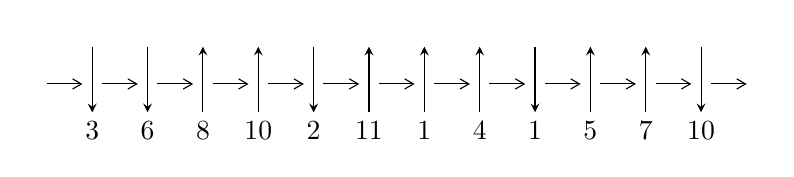
\begin{tikzpicture}[x=20pt, y=17pt]
	% nodes
	\node (C0) at (0, 0) {};
	\node (C1) at (1, 0) {};
	\node (C1U) at (1, +1) {};
	\node (C1D) at (1, -1) {3};

	\node (C2) at (2, 0) {};
	\node (C2U) at (2, +1) {};
	\node (C2D) at (2, -1) {6};

	\node (C3) at (3, 0) {};
	\node (C3U) at (3, +1) {};
	\node (C3D) at (3, -1) {8};

	\node (C4) at (4, 0) {};
	\node (C4U) at (4, +1) {};
	\node (C4D) at (4, -1) {10};

	\node (C5) at (5, 0) {};
	\node (C5U) at (5, +1) {};
	\node (C5D) at (5, -1) {2};

	\node (C6) at (6, 0) {};
	\node (C6U) at (6, +1) {};
	\node (C6D) at (6, -1) {11};

	\node (C7) at (7, 0) {};
	\node (C7U) at (7, +1) {};
	\node (C7D) at (7, -1) {1};

	\node (C8) at (8, 0) {};
	\node (C8U) at (8, +1) {};
	\node (C8D) at (8, -1) {4};

	\node (C9) at (9, 0) {};
	\node (C9U) at (9, +1) {};
	\node (C9D) at (9, -1) {1};

	\node (C10) at (10, 0) {};
	\node (C10U) at (10, +1) {};
	\node (C10D) at (10, -1) {5};

	\node (C11) at (11, 0) {};
	\node (C11U) at (11, +1) {};
	\node (C11D) at (11, -1) {7};

	\node (C12) at (12, 0) {};
	\node (C12U) at (12, +1) {};
	\node (C12D) at (12, -1) {10};
	\node (C13) at (13, 0) {};

	% arrows
	\draw[->,>={angle 60}]
	(C0) edge (C1) (C1) edge (C2) (C2) edge (C3) (C3) edge (C4) (C4) edge (C5) (C5) edge (C6) (C6) edge (C7) (C7) edge (C8) (C8) edge (C9) (C9) edge (C10) (C10) edge (C11) (C11) edge (C12) (C12) edge (C13) ;	\draw[->,>=stealth]
	(C1U) edge (C1D) (C2U) edge (C2D) (C3D) edge (C3U) (C4D) edge (C4U) (C5U) edge (C5D) (C6D) edge (C6U) (C7D) edge (C7U) (C8D) edge (C8U) (C9U) edge (C9D) (C10D) edge (C10U) (C11D) edge (C11U) (C12U) edge (C12D) ;
	\end{tikzpicture} \\
\hhline{~~} \\& 
\textbf{Solving Sequence} \\ \cline{2-2} 
 &
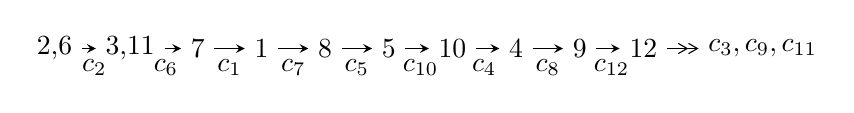
\begin{tikzpicture}[x=23pt, y=7pt]
	% node
	\node (A0) at (-1/8, 0) {2,6};
	\node (A1) at (17/16, 0) {3,11};
	\node (A2) at (17/8, 0) {7};
	\node (A3) at (25/8, 0) {1};
	\node (A4) at (33/8, 0) {8};
	\node (A5) at (41/8, 0) {5};
	\node (A6) at (49/8, 0) {10};
	\node (A7) at (57/8, 0) {4};
	\node (A8) at (65/8, 0) {9};
	\node (A9) at (73/8, 0) {12};
	\node (C1) at (1/2, -1) {$c_{2}$};
	\node (C2) at (13/8, -1) {$c_{6}$};
	\node (C3) at (21/8, -1) {$c_{1}$};
	\node (C4) at (29/8, -1) {$c_{7}$};
	\node (C5) at (37/8, -1) {$c_{5}$};
	\node (C6) at (45/8, -1) {$c_{10}$};
	\node (C7) at (53/8, -1) {$c_{4}$};
	\node (C8) at (61/8, -1) {$c_{8}$};
	\node (C9) at (69/8, -1) {$c_{12}$};
	\node (A10) at (11, 0) {$c_{3},c_{9},c_{11}$};

	% edge
	\draw[->,>=stealth]	
	(A0) edge (A1) (A1) edge (A2) (A2) edge (A3) (A3) edge (A4) (A4) edge (A5) (A5) edge (A6) (A6) edge (A7) (A7) edge (A8) (A8) edge (A9) ;
	\draw[->>,>={angle 60}]	
	(A9) edge (A10);
\end{tikzpicture} \\ 

\end{tabular} \\

\footnotetext{
The image of knot diagram is generated by the software ``\textbf{Draw programme}" developed by Andrew Bartholomew(\url{http://www.layer8.co.uk/maths/draw/index.htm\#Running-draw}), where we modified some parts for our purpose(\url{https://github.com/CATsTAILs/LinksPainter}).
}\phantom \\ \newline 
\centering \textbf{Ideals for irreducible components\footnotemark of $X_{\text{par}}$} 
 
\begin{align*}
I^u_{1}&=\langle 
2.40269\times10^{62} u^{72}-1.72408\times10^{63} u^{71}+\cdots+1.82435\times10^{64} b-1.38356\times10^{64},\\
\phantom{I^u_{1}}&\phantom{= \langle  }2.34275\times10^{62} u^{72}+1.14118\times10^{62} u^{71}+\cdots+4.44964\times10^{62} a+4.68732\times10^{63},\;u^{73}- u^{72}+\cdots+6 u-1\rangle \\
I^u_{2}&=\langle 
u^{19}- u^{18}+\cdots+b-2,\;u^{19}+u^{18}+\cdots+a-6,\;u^{20}-4 u^{18}+\cdots- u+1\rangle \\
\\
\end{align*}
\raggedright * 2 irreducible components of $\dim_{\mathbb{C}}=0$, with total 93 representations.\\
\footnotetext{All coefficients of polynomials are rational numbers. But the coefficients are sometimes approximated in decimal forms when there is not enough margin.}
\newpage
\renewcommand{\arraystretch}{1}
\centering \section*{I. $I^u_{1}= \langle 2.40\times10^{62} u^{72}-1.72\times10^{63} u^{71}+\cdots+1.82\times10^{64} b-1.38\times10^{64},\;2.34\times10^{62} u^{72}+1.14\times10^{62} u^{71}+\cdots+4.45\times10^{62} a+4.69\times10^{63},\;u^{73}- u^{72}+\cdots+6 u-1 \rangle$}
\flushleft \textbf{(i) Arc colorings}\\
\begin{tabular}{m{7pt} m{180pt} m{7pt} m{180pt} }
\flushright $a_{2}=$&$\begin{pmatrix}1\\0\end{pmatrix}$ \\
\flushright $a_{6}=$&$\begin{pmatrix}0\\u\end{pmatrix}$ \\
\flushright $a_{3}=$&$\begin{pmatrix}1\\u^2\end{pmatrix}$ \\
\flushright $a_{11}=$&$\begin{pmatrix}-0.526502 u^{72}-0.256466 u^{71}+\cdots+31.1936 u-10.5341\\-0.0131701 u^{72}+0.0945035 u^{71}+\cdots-9.10210 u+0.758385\end{pmatrix}$ \\
\flushright $a_{7}=$&$\begin{pmatrix}0.429075 u^{72}-0.253130 u^{71}+\cdots+5.78589 u-1.70210\\0.0237826 u^{72}+0.0747905 u^{71}+\cdots-4.64228 u+2.61862\end{pmatrix}$ \\
\flushright $a_{1}=$&$\begin{pmatrix}- u^2+1\\- u^4\end{pmatrix}$ \\
\flushright $a_{8}=$&$\begin{pmatrix}0.354692 u^{72}-0.179230 u^{71}+\cdots+1.83197 u+0.794479\\-0.134146 u^{72}+0.126424 u^{71}+\cdots-4.09974 u+2.52946\end{pmatrix}$ \\
\flushright $a_{5}=$&$\begin{pmatrix}u\\u\end{pmatrix}$ \\
\flushright $a_{10}=$&$\begin{pmatrix}-0.273639 u^{72}-0.495448 u^{71}+\cdots+35.8660 u-11.3984\\0.239693 u^{72}-0.144479 u^{71}+\cdots-4.42963 u-0.105916\end{pmatrix}$ \\
\flushright $a_{4}=$&$\begin{pmatrix}-0.141530 u^{72}+0.130114 u^{71}+\cdots-13.1139 u+4.72440\\0.122092 u^{72}-0.537187 u^{71}+\cdots+8.50726 u-3.27538\end{pmatrix}$ \\
\flushright $a_{9}=$&$\begin{pmatrix}0.0361754 u^{72}+0.773102 u^{71}+\cdots-31.3454 u+11.5188\\-0.219504 u^{72}+0.183374 u^{71}+\cdots+4.64947 u+0.0703768\end{pmatrix}$ \\
\flushright $a_{12}=$&$\begin{pmatrix}-3.01500 u^{72}+3.21861 u^{71}+\cdots-11.8184 u-9.35261\\0.189418 u^{72}-0.0254143 u^{71}+\cdots-9.37084 u+1.71468\end{pmatrix}$\\&\end{tabular}
\flushleft \textbf{(ii) Obstruction class $= -1$}\\~\\
\flushleft \textbf{(iii) Cusp Shapes $= -4.91581 u^{72}+6.79732 u^{71}+\cdots-94.4807 u+6.97585$}\\~\\
\newpage\renewcommand{\arraystretch}{1}
\flushleft \textbf{(iv) u-Polynomials at the component}\newline \\
\begin{tabular}{m{50pt}|m{274pt}}
Crossings & \hspace{64pt}u-Polynomials at each crossing \\
\hline $$\begin{aligned}c_{1}\end{aligned}$$&$\begin{aligned}
&u^{73}+25 u^{72}+\cdots+84 u+1
\end{aligned}$\\
\hline $$\begin{aligned}c_{2},c_{5}\end{aligned}$$&$\begin{aligned}
&u^{73}+u^{72}+\cdots+6 u+1
\end{aligned}$\\
\hline $$\begin{aligned}c_{3},c_{8}\end{aligned}$$&$\begin{aligned}
&u^{73}+u^{72}+\cdots-72 u-29
\end{aligned}$\\
\hline $$\begin{aligned}c_{4},c_{10}\end{aligned}$$&$\begin{aligned}
&u^{73}- u^{72}+\cdots-602 u-2285
\end{aligned}$\\
\hline $$\begin{aligned}c_{6},c_{11}\end{aligned}$$&$\begin{aligned}
&u^{73}- u^{72}+\cdots+6589 u+2209
\end{aligned}$\\
\hline $$\begin{aligned}c_{7}\end{aligned}$$&$\begin{aligned}
&u^{73}-3 u^{72}+\cdots+30630 u-13801
\end{aligned}$\\
\hline $$\begin{aligned}c_{9},c_{12}\end{aligned}$$&$\begin{aligned}
&u^{73}-9 u^{72}+\cdots+42 u-1
\end{aligned}$\\
\hline
\end{tabular}\\~\\
\newpage\renewcommand{\arraystretch}{1}
\flushleft \textbf{(v) Riley Polynomials at the component}\newline \\
\begin{tabular}{m{50pt}|m{274pt}}
Crossings & \hspace{64pt}Riley Polynomials at each crossing \\
\hline $$\begin{aligned}c_{1}\end{aligned}$$&$\begin{aligned}
&y^{73}+55 y^{72}+\cdots+1088 y-1
\end{aligned}$\\
\hline $$\begin{aligned}c_{2},c_{5}\end{aligned}$$&$\begin{aligned}
&y^{73}-25 y^{72}+\cdots+84 y-1
\end{aligned}$\\
\hline $$\begin{aligned}c_{3},c_{8}\end{aligned}$$&$\begin{aligned}
&y^{73}-29 y^{72}+\cdots+20264 y-841
\end{aligned}$\\
\hline $$\begin{aligned}c_{4},c_{10}\end{aligned}$$&$\begin{aligned}
&y^{73}-37 y^{72}+\cdots+153119224 y-5221225
\end{aligned}$\\
\hline $$\begin{aligned}c_{6},c_{11}\end{aligned}$$&$\begin{aligned}
&y^{73}-45 y^{72}+\cdots+119152695 y-4879681
\end{aligned}$\\
\hline $$\begin{aligned}c_{7}\end{aligned}$$&$\begin{aligned}
&y^{73}+11 y^{72}+\cdots-1310013602 y-190467601
\end{aligned}$\\
\hline $$\begin{aligned}c_{9},c_{12}\end{aligned}$$&$\begin{aligned}
&y^{73}-53 y^{72}+\cdots+502 y-1
\end{aligned}$\\
\hline
\end{tabular}\\~\\
\newpage\flushleft \textbf{(vi) Complex Volumes and Cusp Shapes}
$$\begin{array}{c|c|c}  
\text{Solutions to }I^u_{1}& \I (\text{vol} + \sqrt{-1}CS) & \text{Cusp shape}\\
 \hline 
\begin{aligned}
u &= -0.996222 + 0.079970 I \\
a &= -0.640369 + 0.961224 I \\
b &= \phantom{-}0.02392 + 1.95649 I\end{aligned}
 & -5.68162 + 3.39874 I & \phantom{-0.000000 } 0 \\ \hline\begin{aligned}
u &= -0.996222 - 0.079970 I \\
a &= -0.640369 - 0.961224 I \\
b &= \phantom{-}0.02392 - 1.95649 I\end{aligned}
 & -5.68162 - 3.39874 I & \phantom{-0.000000 } 0 \\ \hline\begin{aligned}
u &= -0.758602 + 0.638058 I \\
a &= -0.372335 + 1.210930 I \\
b &= \phantom{-}0.34583 + 1.63890 I\end{aligned}
 & -0.54896 + 3.17316 I & \phantom{-0.000000 } 0 \\ \hline\begin{aligned}
u &= -0.758602 - 0.638058 I \\
a &= -0.372335 - 1.210930 I \\
b &= \phantom{-}0.34583 - 1.63890 I\end{aligned}
 & -0.54896 - 3.17316 I & \phantom{-0.000000 } 0 \\ \hline\begin{aligned}
u &= -0.618315 + 0.821119 I \\
a &= -0.94140 - 1.06158 I \\
b &= \phantom{-}0.088422 - 0.498715 I\end{aligned}
 & \phantom{-}7.38525 - 1.46732 I & \phantom{-0.000000 } 0 \\ \hline\begin{aligned}
u &= -0.618315 - 0.821119 I \\
a &= -0.94140 + 1.06158 I \\
b &= \phantom{-}0.088422 + 0.498715 I\end{aligned}
 & \phantom{-}7.38525 + 1.46732 I & \phantom{-0.000000 } 0 \\ \hline\begin{aligned}
u &= -0.969221\phantom{ +0.000000I} \\
a &= -0.747368\phantom{ +0.000000I} \\
b &= -2.30513\phantom{ +0.000000I}\end{aligned}
 & \phantom{-}4.41153\phantom{ +0.000000I} & -5.41240\phantom{ +0.000000I} \\ \hline\begin{aligned}
u &= \phantom{-}0.751264 + 0.736846 I \\
a &= \phantom{-}1.058580 - 0.390102 I \\
b &= -0.228660 + 0.735522 I\end{aligned}
 & \phantom{-}9.38761 - 0.55526 I & \phantom{-0.000000 } 0 \\ \hline\begin{aligned}
u &= \phantom{-}0.751264 - 0.736846 I \\
a &= \phantom{-}1.058580 + 0.390102 I \\
b &= -0.228660 - 0.735522 I\end{aligned}
 & \phantom{-}9.38761 + 0.55526 I & \phantom{-0.000000 } 0 \\ \hline\begin{aligned}
u &= \phantom{-}0.733170 + 0.756165 I \\
a &= -0.851966 - 1.016840 I \\
b &= -0.109081 - 1.382330 I\end{aligned}
 & -0.08676 + 2.96078 I & \phantom{-0.000000 } 0\\
 \hline 
 \end{array}$$\newpage$$\begin{array}{c|c|c}  
\text{Solutions to }I^u_{1}& \I (\text{vol} + \sqrt{-1}CS) & \text{Cusp shape}\\
 \hline 
\begin{aligned}
u &= \phantom{-}0.733170 - 0.756165 I \\
a &= -0.851966 + 1.016840 I \\
b &= -0.109081 + 1.382330 I\end{aligned}
 & -0.08676 - 2.96078 I & \phantom{-0.000000 } 0 \\ \hline\begin{aligned}
u &= -0.861502 + 0.388627 I \\
a &= \phantom{-}0.165858 + 1.013930 I \\
b &= \phantom{-}0.55739 + 1.55978 I\end{aligned}
 & -0.44770 + 3.61771 I & \phantom{-}3.83289 - 9.05008 I \\ \hline\begin{aligned}
u &= -0.861502 - 0.388627 I \\
a &= \phantom{-}0.165858 - 1.013930 I \\
b &= \phantom{-}0.55739 - 1.55978 I\end{aligned}
 & -0.44770 - 3.61771 I & \phantom{-}3.83289 + 9.05008 I \\ \hline\begin{aligned}
u &= \phantom{-}0.943914 + 0.043003 I \\
a &= -0.918576 + 0.881953 I \\
b &= \phantom{-}0.02090 + 1.95760 I\end{aligned}
 & -4.65821 - 2.86626 I & -1.66244 + 2.85840 I \\ \hline\begin{aligned}
u &= \phantom{-}0.943914 - 0.043003 I \\
a &= -0.918576 - 0.881953 I \\
b &= \phantom{-}0.02090 - 1.95760 I\end{aligned}
 & -4.65821 + 2.86626 I & -1.66244 - 2.85840 I \\ \hline\begin{aligned}
u &= -0.631153 + 0.853761 I \\
a &= \phantom{-}1.204560 + 0.578291 I \\
b &= -0.010140 - 0.154408 I\end{aligned}
 & \phantom{-}2.19037 - 3.39728 I & \phantom{-0.000000 } 0 \\ \hline\begin{aligned}
u &= -0.631153 - 0.853761 I \\
a &= \phantom{-}1.204560 - 0.578291 I \\
b &= -0.010140 + 0.154408 I\end{aligned}
 & \phantom{-}2.19037 + 3.39728 I & \phantom{-0.000000 } 0 \\ \hline\begin{aligned}
u &= \phantom{-}0.892873 + 0.267184 I \\
a &= \phantom{-}0.173653 - 0.505706 I \\
b &= -0.190432 - 0.912777 I\end{aligned}
 & -1.50577 - 0.99916 I & -2.39776 + 0. I\phantom{ +0.000000I} \\ \hline\begin{aligned}
u &= \phantom{-}0.892873 - 0.267184 I \\
a &= \phantom{-}0.173653 + 0.505706 I \\
b &= -0.190432 + 0.912777 I\end{aligned}
 & -1.50577 + 0.99916 I & -2.39776 + 0. I\phantom{ +0.000000I} \\ \hline\begin{aligned}
u &= -0.767998 + 0.745094 I \\
a &= \phantom{-}0.746725 + 0.494096 I \\
b &= -0.01556 + 1.80761 I\end{aligned}
 & \phantom{-}0.46877 - 1.97857 I & \phantom{-0.000000 } 0\\
 \hline 
 \end{array}$$\newpage$$\begin{array}{c|c|c}  
\text{Solutions to }I^u_{1}& \I (\text{vol} + \sqrt{-1}CS) & \text{Cusp shape}\\
 \hline 
\begin{aligned}
u &= -0.767998 - 0.745094 I \\
a &= \phantom{-}0.746725 - 0.494096 I \\
b &= -0.01556 - 1.80761 I\end{aligned}
 & \phantom{-}0.46877 + 1.97857 I & \phantom{-0.000000 } 0 \\ \hline\begin{aligned}
u &= \phantom{-}0.143541 + 0.896389 I \\
a &= -0.216547 - 1.280260 I \\
b &= \phantom{-}0.0239252 - 0.0949787 I\end{aligned}
 & \phantom{-}0.81734 - 5.65289 I & \phantom{-}7.40959 + 5.97302 I \\ \hline\begin{aligned}
u &= \phantom{-}0.143541 - 0.896389 I \\
a &= -0.216547 + 1.280260 I \\
b &= \phantom{-}0.0239252 + 0.0949787 I\end{aligned}
 & \phantom{-}0.81734 + 5.65289 I & \phantom{-}7.40959 - 5.97302 I \\ \hline\begin{aligned}
u &= \phantom{-}0.824608 + 0.727987 I \\
a &= -1.29265 + 0.82770 I \\
b &= -0.231633 + 0.608811 I\end{aligned}
 & \phantom{-}6.55692 - 1.93707 I & \phantom{-0.000000 } 0 \\ \hline\begin{aligned}
u &= \phantom{-}0.824608 - 0.727987 I \\
a &= -1.29265 - 0.82770 I \\
b &= -0.231633 - 0.608811 I\end{aligned}
 & \phantom{-}6.55692 + 1.93707 I & \phantom{-0.000000 } 0 \\ \hline\begin{aligned}
u &= \phantom{-}0.946156 + 0.586430 I \\
a &= \phantom{-}0.432541 - 0.667921 I \\
b &= -0.43463 - 1.49029 I\end{aligned}
 & -2.76173 - 2.00615 I & \phantom{-0.000000 } 0 \\ \hline\begin{aligned}
u &= \phantom{-}0.946156 - 0.586430 I \\
a &= \phantom{-}0.432541 + 0.667921 I \\
b &= -0.43463 + 1.49029 I\end{aligned}
 & -2.76173 + 2.00615 I & \phantom{-0.000000 } 0 \\ \hline\begin{aligned}
u &= -0.343909 + 0.787868 I \\
a &= \phantom{-}0.127670 + 1.043220 I \\
b &= \phantom{-}0.084955 - 0.115660 I\end{aligned}
 & \phantom{-}0.479750 - 0.044976 I & \phantom{-}6.90143 - 1.13729 I \\ \hline\begin{aligned}
u &= -0.343909 - 0.787868 I \\
a &= \phantom{-}0.127670 - 1.043220 I \\
b &= \phantom{-}0.084955 + 0.115660 I\end{aligned}
 & \phantom{-}0.479750 + 0.044976 I & \phantom{-}6.90143 + 1.13729 I \\ \hline\begin{aligned}
u &= -0.937251 + 0.657162 I \\
a &= \phantom{-}1.099920 - 0.537869 I \\
b &= \phantom{-}0.49874 - 1.35415 I\end{aligned}
 & -1.09504 + 1.90890 I & \phantom{-0.000000 } 0\\
 \hline 
 \end{array}$$\newpage$$\begin{array}{c|c|c}  
\text{Solutions to }I^u_{1}& \I (\text{vol} + \sqrt{-1}CS) & \text{Cusp shape}\\
 \hline 
\begin{aligned}
u &= -0.937251 - 0.657162 I \\
a &= \phantom{-}1.099920 + 0.537869 I \\
b &= \phantom{-}0.49874 + 1.35415 I\end{aligned}
 & -1.09504 - 1.90890 I & \phantom{-0.000000 } 0 \\ \hline\begin{aligned}
u &= \phantom{-}0.683384 + 0.923655 I \\
a &= \phantom{-}1.180580 - 0.657252 I \\
b &= -0.0799028 - 0.0563581 I\end{aligned}
 & \phantom{-}4.09129 + 9.93504 I & \phantom{-0.000000 } 0 \\ \hline\begin{aligned}
u &= \phantom{-}0.683384 - 0.923655 I \\
a &= \phantom{-}1.180580 + 0.657252 I \\
b &= -0.0799028 + 0.0563581 I\end{aligned}
 & \phantom{-}4.09129 - 9.93504 I & \phantom{-0.000000 } 0 \\ \hline\begin{aligned}
u &= \phantom{-}0.908958 + 0.710659 I \\
a &= -0.890867 + 1.087230 I \\
b &= -1.09856 + 2.00903 I\end{aligned}
 & \phantom{-}6.29427 - 3.55581 I & \phantom{-0.000000 } 0 \\ \hline\begin{aligned}
u &= \phantom{-}0.908958 - 0.710659 I \\
a &= -0.890867 - 1.087230 I \\
b &= -1.09856 - 2.00903 I\end{aligned}
 & \phantom{-}6.29427 + 3.55581 I & \phantom{-0.000000 } 0 \\ \hline\begin{aligned}
u &= \phantom{-}1.158780 + 0.119477 I \\
a &= -0.690279 + 0.608358 I \\
b &= -1.51845 + 1.26660 I\end{aligned}
 & -4.61256 - 2.51615 I & \phantom{-0.000000 } 0 \\ \hline\begin{aligned}
u &= \phantom{-}1.158780 - 0.119477 I \\
a &= -0.690279 - 0.608358 I \\
b &= -1.51845 - 1.26660 I\end{aligned}
 & -4.61256 + 2.51615 I & \phantom{-0.000000 } 0 \\ \hline\begin{aligned}
u &= -0.809794\phantom{ +0.000000I} \\
a &= \phantom{-}1.59121\phantom{ +0.000000I} \\
b &= \phantom{-}2.15213\phantom{ +0.000000I}\end{aligned}
 & \phantom{-}2.28647\phantom{ +0.000000I} & \phantom{-}3.88350\phantom{ +0.000000I} \\ \hline\begin{aligned}
u &= -0.956447 + 0.710795 I \\
a &= \phantom{-}0.599846 + 0.745235 I \\
b &= -0.60555 + 1.54716 I\end{aligned}
 & -0.11113 + 7.52904 I & \phantom{-0.000000 } 0 \\ \hline\begin{aligned}
u &= -0.956447 - 0.710795 I \\
a &= \phantom{-}0.599846 - 0.745235 I \\
b &= -0.60555 - 1.54716 I\end{aligned}
 & -0.11113 - 7.52904 I & \phantom{-0.000000 } 0\\
 \hline 
 \end{array}$$\newpage$$\begin{array}{c|c|c}  
\text{Solutions to }I^u_{1}& \I (\text{vol} + \sqrt{-1}CS) & \text{Cusp shape}\\
 \hline 
\begin{aligned}
u &= \phantom{-}0.964639 + 0.701087 I \\
a &= \phantom{-}0.340557 - 0.829485 I \\
b &= \phantom{-}1.41277 - 1.84680 I\end{aligned}
 & \phantom{-}8.73288 - 4.94035 I & \phantom{-0.000000 } 0 \\ \hline\begin{aligned}
u &= \phantom{-}0.964639 - 0.701087 I \\
a &= \phantom{-}0.340557 + 0.829485 I \\
b &= \phantom{-}1.41277 + 1.84680 I\end{aligned}
 & \phantom{-}8.73288 + 4.94035 I & \phantom{-0.000000 } 0 \\ \hline\begin{aligned}
u &= \phantom{-}0.853639 + 0.855312 I \\
a &= -1.151840 + 0.283826 I \\
b &= -0.300491 + 0.019376 I\end{aligned}
 & \phantom{-}7.09864 + 0.53230 I & \phantom{-0.000000 } 0 \\ \hline\begin{aligned}
u &= \phantom{-}0.853639 - 0.855312 I \\
a &= -1.151840 - 0.283826 I \\
b &= -0.300491 - 0.019376 I\end{aligned}
 & \phantom{-}7.09864 - 0.53230 I & \phantom{-0.000000 } 0 \\ \hline\begin{aligned}
u &= \phantom{-}0.978323 + 0.710764 I \\
a &= \phantom{-}0.911240 + 0.831323 I \\
b &= \phantom{-}0.43175 + 1.60287 I\end{aligned}
 & -0.83249 - 8.54524 I & \phantom{-0.000000 } 0 \\ \hline\begin{aligned}
u &= \phantom{-}0.978323 - 0.710764 I \\
a &= \phantom{-}0.911240 - 0.831323 I \\
b &= \phantom{-}0.43175 - 1.60287 I\end{aligned}
 & -0.83249 + 8.54524 I & \phantom{-0.000000 } 0 \\ \hline\begin{aligned}
u &= -1.189080 + 0.229032 I \\
a &= -0.808750 - 0.686874 I \\
b &= -1.52953 - 1.44010 I\end{aligned}
 & -3.81596 + 9.32233 I & \phantom{-0.000000 } 0 \\ \hline\begin{aligned}
u &= -1.189080 - 0.229032 I \\
a &= -0.808750 + 0.686874 I \\
b &= -1.52953 + 1.44010 I\end{aligned}
 & -3.81596 - 9.32233 I & \phantom{-0.000000 } 0 \\ \hline\begin{aligned}
u &= \phantom{-}1.22912\phantom{ +0.000000I} \\
a &= \phantom{-}1.00223\phantom{ +0.000000I} \\
b &= \phantom{-}1.54563\phantom{ +0.000000I}\end{aligned}
 & \phantom{-}0.994441\phantom{ +0.000000I} & \phantom{-0.000000 } 0 \\ \hline\begin{aligned}
u &= \phantom{-}0.557309 + 0.526306 I \\
a &= \phantom{-}0.544371 - 0.023747 I \\
b &= -0.148793 - 1.306520 I\end{aligned}
 & -1.71887 - 2.44461 I & \phantom{-}5.05962 + 1.77262 I\\
 \hline 
 \end{array}$$\newpage$$\begin{array}{c|c|c}  
\text{Solutions to }I^u_{1}& \I (\text{vol} + \sqrt{-1}CS) & \text{Cusp shape}\\
 \hline 
\begin{aligned}
u &= \phantom{-}0.557309 - 0.526306 I \\
a &= \phantom{-}0.544371 + 0.023747 I \\
b &= -0.148793 + 1.306520 I\end{aligned}
 & -1.71887 + 2.44461 I & \phantom{-}5.05962 - 1.77262 I \\ \hline\begin{aligned}
u &= -0.846572 + 0.914565 I \\
a &= -0.655447 - 0.508702 I \\
b &= \phantom{-}0.167328 - 0.162277 I\end{aligned}
 & \phantom{-}7.36439 + 2.36950 I & \phantom{-0.000000 } 0 \\ \hline\begin{aligned}
u &= -0.846572 - 0.914565 I \\
a &= -0.655447 + 0.508702 I \\
b &= \phantom{-}0.167328 + 0.162277 I\end{aligned}
 & \phantom{-}7.36439 - 2.36950 I & \phantom{-0.000000 } 0 \\ \hline\begin{aligned}
u &= -1.106920 + 0.577507 I \\
a &= \phantom{-}0.548477 + 0.039525 I \\
b &= \phantom{-}1.248990 + 0.006219 I\end{aligned}
 & -1.75051 + 5.10682 I & \phantom{-0.000000 } 0 \\ \hline\begin{aligned}
u &= -1.106920 - 0.577507 I \\
a &= \phantom{-}0.548477 - 0.039525 I \\
b &= \phantom{-}1.248990 - 0.006219 I\end{aligned}
 & -1.75051 - 5.10682 I & \phantom{-0.000000 } 0 \\ \hline\begin{aligned}
u &= \phantom{-}0.948038 + 0.819646 I \\
a &= -0.268358 + 1.134470 I \\
b &= -0.50120 + 1.94706 I\end{aligned}
 & \phantom{-}6.80244 - 6.76181 I & \phantom{-0.000000 } 0 \\ \hline\begin{aligned}
u &= \phantom{-}0.948038 - 0.819646 I \\
a &= -0.268358 - 1.134470 I \\
b &= -0.50120 - 1.94706 I\end{aligned}
 & \phantom{-}6.80244 + 6.76181 I & \phantom{-0.000000 } 0 \\ \hline\begin{aligned}
u &= \phantom{-}1.183950 + 0.434407 I \\
a &= \phantom{-}0.750592 - 0.018384 I \\
b &= \phantom{-}1.351730 + 0.004092 I\end{aligned}
 & -2.58515 + 0.91174 I & \phantom{-0.000000 } 0 \\ \hline\begin{aligned}
u &= \phantom{-}1.183950 - 0.434407 I \\
a &= \phantom{-}0.750592 + 0.018384 I \\
b &= \phantom{-}1.351730 - 0.004092 I\end{aligned}
 & -2.58515 - 0.91174 I & \phantom{-0.000000 } 0 \\ \hline\begin{aligned}
u &= -1.047120 + 0.715765 I \\
a &= -0.832244 - 0.806720 I \\
b &= -1.12523 - 1.67057 I\end{aligned}
 & \phantom{-}6.11341 + 7.23773 I & \phantom{-0.000000 } 0\\
 \hline 
 \end{array}$$\newpage$$\begin{array}{c|c|c}  
\text{Solutions to }I^u_{1}& \I (\text{vol} + \sqrt{-1}CS) & \text{Cusp shape}\\
 \hline 
\begin{aligned}
u &= -1.047120 - 0.715765 I \\
a &= -0.832244 + 0.806720 I \\
b &= -1.12523 + 1.67057 I\end{aligned}
 & \phantom{-}6.11341 - 7.23773 I & \phantom{-0.000000 } 0 \\ \hline\begin{aligned}
u &= -1.051990 + 0.719300 I \\
a &= \phantom{-}0.446861 + 1.074860 I \\
b &= \phantom{-}1.06139 + 2.17386 I\end{aligned}
 & \phantom{-}0.91326 + 9.25948 I & \phantom{-0.000000 } 0 \\ \hline\begin{aligned}
u &= -1.051990 - 0.719300 I \\
a &= \phantom{-}0.446861 - 1.074860 I \\
b &= \phantom{-}1.06139 - 2.17386 I\end{aligned}
 & \phantom{-}0.91326 - 9.25948 I & \phantom{-0.000000 } 0 \\ \hline\begin{aligned}
u &= -0.977624 + 0.850736 I \\
a &= -0.417028 - 0.618249 I \\
b &= -0.65490 - 1.45884 I\end{aligned}
 & \phantom{-}6.94563 + 4.12886 I & \phantom{-0.000000 } 0 \\ \hline\begin{aligned}
u &= -0.977624 - 0.850736 I \\
a &= -0.417028 + 0.618249 I \\
b &= -0.65490 + 1.45884 I\end{aligned}
 & \phantom{-}6.94563 - 4.12886 I & \phantom{-0.000000 } 0 \\ \hline\begin{aligned}
u &= \phantom{-}1.062780 + 0.766541 I \\
a &= \phantom{-}0.558144 - 1.091810 I \\
b &= \phantom{-}1.05492 - 2.27168 I\end{aligned}
 & \phantom{-}2.9062 - 16.1647 I & \phantom{-0.000000 } 0 \\ \hline\begin{aligned}
u &= \phantom{-}1.062780 - 0.766541 I \\
a &= \phantom{-}0.558144 + 1.091810 I \\
b &= \phantom{-}1.05492 + 2.27168 I\end{aligned}
 & \phantom{-}2.9062 + 16.1647 I & \phantom{-0.000000 } 0 \\ \hline\begin{aligned}
u &= -0.624370\phantom{ +0.000000I} \\
a &= \phantom{-}2.54662\phantom{ +0.000000I} \\
b &= \phantom{-}0.805344\phantom{ +0.000000I}\end{aligned}
 & \phantom{-}3.04322\phantom{ +0.000000I} & -5.86610\phantom{ +0.000000I} \\ \hline\begin{aligned}
u &= -0.362561 + 0.439077 I \\
a &= \phantom{-}0.900518 + 0.463831 I \\
b &= \phantom{-}0.193003 - 0.160197 I\end{aligned}
 & \phantom{-}1.059400 - 0.337570 I & \phantom{-}9.21872 + 1.59251 I \\ \hline\begin{aligned}
u &= -0.362561 - 0.439077 I \\
a &= \phantom{-}0.900518 - 0.463831 I \\
b &= \phantom{-}0.193003 + 0.160197 I\end{aligned}
 & \phantom{-}1.059400 + 0.337570 I & \phantom{-}9.21872 - 1.59251 I\\
 \hline 
 \end{array}$$\newpage$$\begin{array}{c|c|c}  
\text{Solutions to }I^u_{1}& \I (\text{vol} + \sqrt{-1}CS) & \text{Cusp shape}\\
 \hline 
\begin{aligned}
u &= -0.318447\phantom{ +0.000000I} \\
a &= -3.97650\phantom{ +0.000000I} \\
b &= \phantom{-}0.921377\phantom{ +0.000000I}\end{aligned}
 & \phantom{-}6.81257\phantom{ +0.000000I} & \phantom{-}17.0470\phantom{ +0.000000I} \\ \hline\begin{aligned}
u &= \phantom{-}0.164283 + 0.047310 I \\
a &= -0.05014 + 4.02701 I \\
b &= -1.34290 - 0.64628 I\end{aligned}
 & -2.12942 - 2.53807 I & -0.97059 + 1.61971 I \\ \hline\begin{aligned}
u &= \phantom{-}0.164283 - 0.047310 I \\
a &= -0.05014 - 4.02701 I \\
b &= -1.34290 + 0.64628 I\end{aligned}
 & -2.12942 + 2.53807 I & -0.97059 - 1.61971 I\\
 \hline 
 \end{array}$$\newpage\newpage\renewcommand{\arraystretch}{1}
\centering \section*{II. $I^u_{2}= \langle u^{19}- u^{18}+\cdots+b-2,\;u^{19}+u^{18}+\cdots+a-6,\;u^{20}-4 u^{18}+\cdots- u+1 \rangle$}
\flushleft \textbf{(i) Arc colorings}\\
\begin{tabular}{m{7pt} m{180pt} m{7pt} m{180pt} }
\flushright $a_{2}=$&$\begin{pmatrix}1\\0\end{pmatrix}$ \\
\flushright $a_{6}=$&$\begin{pmatrix}0\\u\end{pmatrix}$ \\
\flushright $a_{3}=$&$\begin{pmatrix}1\\u^2\end{pmatrix}$ \\
\flushright $a_{11}=$&$\begin{pmatrix}- u^{19}- u^{18}+\cdots+u+6\\- u^{19}+u^{18}+\cdots+4 u+2\end{pmatrix}$ \\
\flushright $a_{7}=$&$\begin{pmatrix}-5 u^{19}- u^{18}+\cdots+12 u+6\\-2 u^{19}- u^{18}+\cdots+2 u+5\end{pmatrix}$ \\
\flushright $a_{1}=$&$\begin{pmatrix}- u^2+1\\- u^4\end{pmatrix}$ \\
\flushright $a_{8}=$&$\begin{pmatrix}-6 u^{19}-2 u^{18}+\cdots+13 u+9\\-2 u^{19}- u^{18}+\cdots+u+5\end{pmatrix}$ \\
\flushright $a_{5}=$&$\begin{pmatrix}u\\u\end{pmatrix}$ \\
\flushright $a_{10}=$&$\begin{pmatrix}- u^{19}-2 u^{18}+\cdots- u+8\\- u^{19}+4 u^{17}+\cdots+2 u+4\end{pmatrix}$ \\
\flushright $a_{4}=$&$\begin{pmatrix}4 u^{19}-15 u^{17}+\cdots-14 u-1\\u^{15}-3 u^{13}+\cdots-3 u-1\end{pmatrix}$ \\
\flushright $a_{9}=$&$\begin{pmatrix}-2 u^{19}-3 u^{18}+\cdots-43 u^2+11\\- u^{19}+4 u^{17}+\cdots+2 u+4\end{pmatrix}$ \\
\flushright $a_{12}=$&$\begin{pmatrix}4 u^{19}+3 u^{18}+\cdots-4 u-8\\3 u^{19}+2 u^{18}+\cdots-3 u-3\end{pmatrix}$\\&\end{tabular}
\flushleft \textbf{(ii) Obstruction class $= 1$}\\~\\
\flushleft \textbf{(iii) Cusp Shapes $= -20 u^{19}-8 u^{18}+71 u^{17}+50 u^{16}-199 u^{15}-141 u^{14}+362 u^{13}+309 u^{12}-520 u^{11}-465 u^{10}+557 u^9+555 u^8-458 u^7-481 u^6+268 u^5+302 u^4-86 u^3-110 u^2+29 u+24$}\\~\\
\newpage\renewcommand{\arraystretch}{1}
\flushleft \textbf{(iv) u-Polynomials at the component}\newline \\
\begin{tabular}{m{50pt}|m{274pt}}
Crossings & \hspace{64pt}u-Polynomials at each crossing \\
\hline $$\begin{aligned}c_{1}\end{aligned}$$&$\begin{aligned}
&u^{20}-8 u^{19}+\cdots-13 u+1
\end{aligned}$\\
\hline $$\begin{aligned}c_{2}\end{aligned}$$&$\begin{aligned}
&u^{20}-4 u^{18}+\cdots- u+1
\end{aligned}$\\
\hline $$\begin{aligned}c_{3}\end{aligned}$$&$\begin{aligned}
&u^{20}-8 u^{18}+\cdots+u+1
\end{aligned}$\\
\hline $$\begin{aligned}c_{4}\end{aligned}$$&$\begin{aligned}
&u^{20}-6 u^{18}+\cdots- u+1
\end{aligned}$\\
\hline $$\begin{aligned}c_{5}\end{aligned}$$&$\begin{aligned}
&u^{20}-4 u^{18}+\cdots+u+1
\end{aligned}$\\
\hline $$\begin{aligned}c_{6}\end{aligned}$$&$\begin{aligned}
&u^{20}+4 u^{19}+\cdots+4 u+1
\end{aligned}$\\
\hline $$\begin{aligned}c_{7}\end{aligned}$$&$\begin{aligned}
&u^{20}-2 u^{18}+\cdots-343 u+37
\end{aligned}$\\
\hline $$\begin{aligned}c_{8}\end{aligned}$$&$\begin{aligned}
&u^{20}-8 u^{18}+\cdots- u+1
\end{aligned}$\\
\hline $$\begin{aligned}c_{9}\end{aligned}$$&$\begin{aligned}
&u^{20}-4 u^{19}+\cdots+11 u-1
\end{aligned}$\\
\hline $$\begin{aligned}c_{10}\end{aligned}$$&$\begin{aligned}
&u^{20}-6 u^{18}+\cdots+u+1
\end{aligned}$\\
\hline $$\begin{aligned}c_{11}\end{aligned}$$&$\begin{aligned}
&u^{20}-4 u^{19}+\cdots-4 u+1
\end{aligned}$\\
\hline $$\begin{aligned}c_{12}\end{aligned}$$&$\begin{aligned}
&u^{20}+4 u^{19}+\cdots-11 u-1
\end{aligned}$\\
\hline
\end{tabular}\\~\\
\newpage\renewcommand{\arraystretch}{1}
\flushleft \textbf{(v) Riley Polynomials at the component}\newline \\
\begin{tabular}{m{50pt}|m{274pt}}
Crossings & \hspace{64pt}Riley Polynomials at each crossing \\
\hline $$\begin{aligned}c_{1}\end{aligned}$$&$\begin{aligned}
&y^{20}+16 y^{19}+\cdots-13 y+1
\end{aligned}$\\
\hline $$\begin{aligned}c_{2},c_{5}\end{aligned}$$&$\begin{aligned}
&y^{20}-8 y^{19}+\cdots-13 y+1
\end{aligned}$\\
\hline $$\begin{aligned}c_{3},c_{8}\end{aligned}$$&$\begin{aligned}
&y^{20}-16 y^{19}+\cdots-21 y+1
\end{aligned}$\\
\hline $$\begin{aligned}c_{4},c_{10}\end{aligned}$$&$\begin{aligned}
&y^{20}-12 y^{19}+\cdots+3 y+1
\end{aligned}$\\
\hline $$\begin{aligned}c_{6},c_{11}\end{aligned}$$&$\begin{aligned}
&y^{20}-16 y^{19}+\cdots+4 y+1
\end{aligned}$\\
\hline $$\begin{aligned}c_{7}\end{aligned}$$&$\begin{aligned}
&y^{20}-4 y^{19}+\cdots-48311 y+1369
\end{aligned}$\\
\hline $$\begin{aligned}c_{9},c_{12}\end{aligned}$$&$\begin{aligned}
&y^{20}-8 y^{19}+\cdots-139 y+1
\end{aligned}$\\
\hline
\end{tabular}\\~\\
\newpage\flushleft \textbf{(vi) Complex Volumes and Cusp Shapes}
$$\begin{array}{c|c|c}  
\text{Solutions to }I^u_{2}& \I (\text{vol} + \sqrt{-1}CS) & \text{Cusp shape}\\
 \hline 
\begin{aligned}
u &= -0.942703\phantom{ +0.000000I} \\
a &= \phantom{-}1.01394\phantom{ +0.000000I} \\
b &= \phantom{-}2.46434\phantom{ +0.000000I}\end{aligned}
 & \phantom{-}4.96957\phantom{ +0.000000I} & \phantom{-}9.67670\phantom{ +0.000000I} \\ \hline\begin{aligned}
u &= \phantom{-}1.021990 + 0.401552 I \\
a &= \phantom{-}0.490770 + 0.256167 I \\
b &= \phantom{-}0.324519 - 0.338569 I\end{aligned}
 & -3.43274 - 0.00501 I & -0.269919 + 0.886126 I \\ \hline\begin{aligned}
u &= \phantom{-}1.021990 - 0.401552 I \\
a &= \phantom{-}0.490770 - 0.256167 I \\
b &= \phantom{-}0.324519 + 0.338569 I\end{aligned}
 & -3.43274 + 0.00501 I & -0.269919 - 0.886126 I \\ \hline\begin{aligned}
u &= -0.676743 + 0.574335 I \\
a &= -0.665466 + 0.475040 I \\
b &= -1.05039 + 1.39641 I\end{aligned}
 & -1.31380 - 1.46689 I & \phantom{-}1.93443 - 1.03956 I \\ \hline\begin{aligned}
u &= -0.676743 - 0.574335 I \\
a &= -0.665466 - 0.475040 I \\
b &= -1.05039 - 1.39641 I\end{aligned}
 & -1.31380 + 1.46689 I & \phantom{-}1.93443 + 1.03956 I \\ \hline\begin{aligned}
u &= \phantom{-}0.811874 + 0.794873 I \\
a &= -0.956293 + 0.516230 I \\
b &= \phantom{-}0.278281 - 0.253589 I\end{aligned}
 & \phantom{-}10.29410 - 1.34128 I & \phantom{-}11.37265 + 3.04262 I \\ \hline\begin{aligned}
u &= \phantom{-}0.811874 - 0.794873 I \\
a &= -0.956293 - 0.516230 I \\
b &= \phantom{-}0.278281 + 0.253589 I\end{aligned}
 & \phantom{-}10.29410 + 1.34128 I & \phantom{-}11.37265 - 3.04262 I \\ \hline\begin{aligned}
u &= \phantom{-}1.14495\phantom{ +0.000000I} \\
a &= \phantom{-}1.07374\phantom{ +0.000000I} \\
b &= \phantom{-}1.53754\phantom{ +0.000000I}\end{aligned}
 & \phantom{-}0.705306\phantom{ +0.000000I} & -7.89590\phantom{ +0.000000I} \\ \hline\begin{aligned}
u &= -1.011460 + 0.552332 I \\
a &= \phantom{-}0.125011 - 0.483876 I \\
b &= -0.386024 - 0.055826 I\end{aligned}
 & -2.42227 + 5.99613 I & \phantom{-}1.25444 - 6.99994 I \\ \hline\begin{aligned}
u &= -1.011460 - 0.552332 I \\
a &= \phantom{-}0.125011 + 0.483876 I \\
b &= -0.386024 + 0.055826 I\end{aligned}
 & -2.42227 - 5.99613 I & \phantom{-}1.25444 + 6.99994 I\\
 \hline 
 \end{array}$$\newpage$$\begin{array}{c|c|c}  
\text{Solutions to }I^u_{2}& \I (\text{vol} + \sqrt{-1}CS) & \text{Cusp shape}\\
 \hline 
\begin{aligned}
u &= -0.808558 + 0.852100 I \\
a &= -1.110280 - 0.654219 I \\
b &= -0.324330 - 0.410095 I\end{aligned}
 & \phantom{-}7.38412 + 0.35956 I & \phantom{-}10.74792 - 1.94607 I \\ \hline\begin{aligned}
u &= -0.808558 - 0.852100 I \\
a &= -1.110280 + 0.654219 I \\
b &= -0.324330 + 0.410095 I\end{aligned}
 & \phantom{-}7.38412 - 0.35956 I & \phantom{-}10.74792 + 1.94607 I \\ \hline\begin{aligned}
u &= \phantom{-}0.958262 + 0.756351 I \\
a &= -0.497932 + 0.796929 I \\
b &= -1.25854 + 1.82161 I\end{aligned}
 & \phantom{-}9.83772 - 4.51280 I & \phantom{-}11.07027 + 3.02713 I \\ \hline\begin{aligned}
u &= \phantom{-}0.958262 - 0.756351 I \\
a &= -0.497932 - 0.796929 I \\
b &= -1.25854 - 1.82161 I\end{aligned}
 & \phantom{-}9.83772 + 4.51280 I & \phantom{-}11.07027 - 3.02713 I \\ \hline\begin{aligned}
u &= \phantom{-}0.632431 + 0.395728 I \\
a &= \phantom{-}0.029010 - 1.115310 I \\
b &= -0.61602 - 2.06351 I\end{aligned}
 & -2.02985 - 3.37926 I & -0.02656 + 9.44485 I \\ \hline\begin{aligned}
u &= \phantom{-}0.632431 - 0.395728 I \\
a &= \phantom{-}0.029010 + 1.115310 I \\
b &= -0.61602 + 2.06351 I\end{aligned}
 & -2.02985 + 3.37926 I & -0.02656 - 9.44485 I \\ \hline\begin{aligned}
u &= -0.981912 + 0.806314 I \\
a &= -0.565494 - 0.975827 I \\
b &= -0.72422 - 1.69291 I\end{aligned}
 & \phantom{-}6.85419 + 5.82262 I & \phantom{-}8.97131 - 3.20438 I \\ \hline\begin{aligned}
u &= -0.981912 - 0.806314 I \\
a &= -0.565494 + 0.975827 I \\
b &= -0.72422 + 1.69291 I\end{aligned}
 & \phantom{-}6.85419 - 5.82262 I & \phantom{-}8.97131 + 3.20438 I \\ \hline\begin{aligned}
u &= -0.603876\phantom{ +0.000000I} \\
a &= \phantom{-}2.10690\phantom{ +0.000000I} \\
b &= -0.708769\phantom{ +0.000000I}\end{aligned}
 & \phantom{-}6.39267\phantom{ +0.000000I} & -2.87160\phantom{ +0.000000I} \\ \hline\begin{aligned}
u &= \phantom{-}0.509858\phantom{ +0.000000I} \\
a &= \phantom{-}3.10678\phantom{ +0.000000I} \\
b &= \phantom{-}1.22034\phantom{ +0.000000I}\end{aligned}
 & \phantom{-}3.38690\phantom{ +0.000000I} & \phantom{-}18.9820\phantom{ +0.000000I}\\
 \hline 
 \end{array}$$\newpage
\newpage\renewcommand{\arraystretch}{1}
\centering \section*{ III. u-Polynomials}
\begin{tabular}{m{50pt}|m{274pt}}
Crossings & \hspace{64pt}u-Polynomials at each crossing \\
\hline $$\begin{aligned}c_{1}\end{aligned}$$&$\begin{aligned}
&(u^{20}-8 u^{19}+\cdots-13 u+1)(u^{73}+25 u^{72}+\cdots+84 u+1)
\end{aligned}$\\
\hline $$\begin{aligned}c_{2}\end{aligned}$$&$\begin{aligned}
&(u^{20}-4 u^{18}+\cdots- u+1)(u^{73}+u^{72}+\cdots+6 u+1)
\end{aligned}$\\
\hline $$\begin{aligned}c_{3}\end{aligned}$$&$\begin{aligned}
&(u^{20}-8 u^{18}+\cdots+u+1)(u^{73}+u^{72}+\cdots-72 u-29)
\end{aligned}$\\
\hline $$\begin{aligned}c_{4}\end{aligned}$$&$\begin{aligned}
&(u^{20}-6 u^{18}+\cdots- u+1)(u^{73}- u^{72}+\cdots-602 u-2285)
\end{aligned}$\\
\hline $$\begin{aligned}c_{5}\end{aligned}$$&$\begin{aligned}
&(u^{20}-4 u^{18}+\cdots+u+1)(u^{73}+u^{72}+\cdots+6 u+1)
\end{aligned}$\\
\hline $$\begin{aligned}c_{6}\end{aligned}$$&$\begin{aligned}
&(u^{20}+4 u^{19}+\cdots+4 u+1)(u^{73}- u^{72}+\cdots+6589 u+2209)
\end{aligned}$\\
\hline $$\begin{aligned}c_{7}\end{aligned}$$&$\begin{aligned}
&(u^{20}-2 u^{18}+\cdots-343 u+37)(u^{73}-3 u^{72}+\cdots+30630 u-13801)
\end{aligned}$\\
\hline $$\begin{aligned}c_{8}\end{aligned}$$&$\begin{aligned}
&(u^{20}-8 u^{18}+\cdots- u+1)(u^{73}+u^{72}+\cdots-72 u-29)
\end{aligned}$\\
\hline $$\begin{aligned}c_{9}\end{aligned}$$&$\begin{aligned}
&(u^{20}-4 u^{19}+\cdots+11 u-1)(u^{73}-9 u^{72}+\cdots+42 u-1)
\end{aligned}$\\
\hline $$\begin{aligned}c_{10}\end{aligned}$$&$\begin{aligned}
&(u^{20}-6 u^{18}+\cdots+u+1)(u^{73}- u^{72}+\cdots-602 u-2285)
\end{aligned}$\\
\hline $$\begin{aligned}c_{11}\end{aligned}$$&$\begin{aligned}
&(u^{20}-4 u^{19}+\cdots-4 u+1)(u^{73}- u^{72}+\cdots+6589 u+2209)
\end{aligned}$\\
\hline $$\begin{aligned}c_{12}\end{aligned}$$&$\begin{aligned}
&(u^{20}+4 u^{19}+\cdots-11 u-1)(u^{73}-9 u^{72}+\cdots+42 u-1)
\end{aligned}$\\
\hline
\end{tabular}\newpage\renewcommand{\arraystretch}{1}
\centering \section*{ IV. Riley Polynomials}
\begin{tabular}{m{50pt}|m{274pt}}
Crossings & \hspace{64pt}Riley Polynomials at each crossing \\
\hline $$\begin{aligned}c_{1}\end{aligned}$$&$\begin{aligned}
&(y^{20}+16 y^{19}+\cdots-13 y+1)(y^{73}+55 y^{72}+\cdots+1088 y-1)
\end{aligned}$\\
\hline $$\begin{aligned}c_{2},c_{5}\end{aligned}$$&$\begin{aligned}
&(y^{20}-8 y^{19}+\cdots-13 y+1)(y^{73}-25 y^{72}+\cdots+84 y-1)
\end{aligned}$\\
\hline $$\begin{aligned}c_{3},c_{8}\end{aligned}$$&$\begin{aligned}
&(y^{20}-16 y^{19}+\cdots-21 y+1)(y^{73}-29 y^{72}+\cdots+20264 y-841)
\end{aligned}$\\
\hline $$\begin{aligned}c_{4},c_{10}\end{aligned}$$&$\begin{aligned}
&(y^{20}-12 y^{19}+\cdots+3 y+1)\\
&\cdot(y^{73}-37 y^{72}+\cdots+153119224 y-5221225)
\end{aligned}$\\
\hline $$\begin{aligned}c_{6},c_{11}\end{aligned}$$&$\begin{aligned}
&(y^{20}-16 y^{19}+\cdots+4 y+1)\\
&\cdot(y^{73}-45 y^{72}+\cdots+119152695 y-4879681)
\end{aligned}$\\
\hline $$\begin{aligned}c_{7}\end{aligned}$$&$\begin{aligned}
&(y^{20}-4 y^{19}+\cdots-48311 y+1369)\\
&\cdot(y^{73}+11 y^{72}+\cdots-1310013602 y-190467601)
\end{aligned}$\\
\hline $$\begin{aligned}c_{9},c_{12}\end{aligned}$$&$\begin{aligned}
&(y^{20}-8 y^{19}+\cdots-139 y+1)(y^{73}-53 y^{72}+\cdots+502 y-1)
\end{aligned}$\\
\hline
\end{tabular}
\vskip 2pc
\end{document}